%!TEX TS-program = xelatex
%!TEX encoding = UTF-8 Unicode

\documentclass[12pt, a4paper]{article}

%% Page Layout
\usepackage[margin=2.54cm]{geometry}

\usepackage{enumitem}

% \usepackage{euler} % math font package needs to be loaded before others
\usepackage{xunicode,xltxtra, polyglossia}
\setdefaultlanguage[variant=american]{english}

%% fonts, symbols, text
	%%% fonts
	\usepackage{fontspec} %(include if mathspec is not loaded)
	\defaultfontfeatures{Mapping=tex-text, Ligatures=TeX}
	%%% text decoration
	\usepackage[normalem]{ulem} % sout
	%%% semantics symbols
	\usepackage{stmaryrd}
	\usepackage{amsmath,amssymb}
	\newcommand{\transl}{\rightsquigarrow \ensuremath}
	%%% other symbols
	\usepackage{pifont}% http://ctan.org/pkg/pifont
	\newcommand{\cmark}{\ding{51}}%
	\newcommand{\xmark}{\ding{55}}%

%% layout
%%% page layout
\usepackage{multicol}

%% bibliography
	\usepackage[round]{natbib}
	\newcommand{\posscite}[1]{\citeauthor{#1}'s (\citeyear{#1})}
	\renewcommand*{\refname}{\normalsize\textbf{References}\\ \vspace{-.5\baselineskip}}
	\newcommand{\citepos}[1]{\citeauthor{#1}'s \citeyear{\#1}}
	\newcommand{\citeposs}[1]{\citeauthor{#1}'s}
	\newcommand{\citetpos}[1]{\citeauthor{#1}'s (\citeyear{\#1})}

%% figures, examples, diagrams
	%%% examples
	\usepackage{linguex}
	\renewcommand{\firstrefdash}{}
	%%% tables 
	\usepackage{booktabs}
	%%% figures
	\usepackage{graphics}


%% decoration and features
%%% colors
\usepackage[dvipsnames]{xcolor}

%% fonts
	\setmainfont[Scale=MatchLowercase,Mapping=tex-text, SmallCapsFeatures={Letters=SmallCaps}]{Times New Roman}
	\setsansfont[Scale=MatchLowercase,Mapping=tex-text]{Times New Roman}
	\setmonofont[Scale=MatchLowercase]{Andale Mono}

% spacing
	\parindent=2ex

\begin{document}

\bibliographystyle{plainnat}
% \enablehyphenation
% \vspace{-2em}
% \maketitle

\begin{center}
	\textbf{\large%\thetitle
		Projection variability of attitude complements across different operators}
\end{center}

\vspace{-.7\baselineskip}
\noindent 
	We present experimental data that the projection of the content of attitude complements \textbf{(i)} varies between entailment-canceling operators, and \textbf{(ii)} that this by-operator variation differs between attitude predicates.
	%
	The observed variability is not captured by existing theoretical accounts of projection
	(e.g., \citealt{heim_projection_1983,van_der_sandt_presupposition_1992,abrusan_predicting_2011,schlenker_triggering_2021}), but suggests that an analysis must consider interactions between predicates and operators, which cannot be fully determined by lexical classes. Instead, our results reveal a more nuanced picture of lexical semantic and pragmatic properties, which raises important questions for future research on projection.
	%
	
\noindent {\bf Projection across entailment-cancelling operators.}
	Language users may infer that a speaker who utters an attitude ascription, as in \ref{ex:family}, is committed to the content of the complement (CC),
	even when it occurs under an entailment-canceling operator, like negation \ref{ex:neg}, polar questions \ref{ex:q}, modals \ref{ex:mod}, or conditionals \ref{ex:cond}, in which case we say that it \emph{projects}.

	\vspace{-.5\baselineskip}
	\ex. \label{ex:family}
		\a. \label{ex:neg}
			{\bf Negation:} \hfill
			\emph{\lq Cole didn't discover that Julian dances salsa.\rq}
		\b. \label{ex:q}
			{\bf Polar Question:} \hfill
			\emph{\lq Did Cole discover that Julian dances salsa?\rq}
		\c. \label{ex:mod}
			{\bf Modal:} \hfill
			\emph{\lq Perhaps Cole discovered that Julian dances salsa.\rq}
		\d. \label{ex:cond}
			{\bf Conditional:} \hfill
			\emph{\lq If Cole discovered that Julian dances salsa, Logan will be joyful.\rq}
		\z.
	\z.
	

	\vspace{-.5\baselineskip}
	\noindent  Current research only rarely examines differences in projectivity across these four operators, with conflicting findings.
	%
	\citet{smith_relationship_2014} found that that the content of non-restrictive relative clauses and the preparatory content of \emph{win} was more projective under conditionals than negation, whereas the projective content of epithets and the clausal complement of \emph{know} showed the opposite pattern.
	%
	\citet{karttunen_observations_1971} proposed that the CC of English factive predicates (e.g. \emph{be annoyed, regret}) projects across all four operators, whereas that of semi-factives (e.g. \emph{discover, realize, see, notice}) only projects across negation.
	%
	In contrast, \posscite{sieker_projective_2022} investigation of the projection of the CC of German attitude predicates found higher projectivity under negation than other operators (e.g. modals), but no interaction with predicate type. In particular, they did not find a difference between factive and semi-factive verbs, nor did they replicate \posscite{smith_relationship_2014} result for the German counterpart of `know' (\emph{wissen}).
	%
	The divergent results raise the question of whether they are due to variation between English and German or methodological differences.


\noindent
{\bfseries Experiment.}
	%
	We conducted a series of experiments designed to investigate projection from under the four entailment-canceling operators in \ref{ex:family}, using the `certain that' diagnostic (see e.g., \citealp{tonhauser_how_2018,djarv_prosodic_2017,mahler_social_2020,sieker_projective_2022}). We applied this diagnostic to the contents of the complements of 20 English clause-embedding predicates, including purported factive predicates (e.g., \emph{be annoyed, know, reveal}) and purported semi-factive predicates (e.g., \emph{discover, see}),
	as well as 15 non-factive predicates, due to recent findings that their complements are also projective, albeit to varying degrees (\citealt{degen_are_2022}).

\noindent 
{\bf Methods and Expectations.}
	Projection of the CC of the 20 attitude predicates was measured in four sets of experiments: The predicates were embedded in polar questions in Exps.~1, under negation (Exps.~2), under {\em perhaps} (Exps.~3), and in conditional antecedents (Exps.~4). (Each set of experiments contained three experiments differing in an at-issueness measure used in a separate block. We focus on the projection ratings here.) In each experiment, participants read utterances like those in \ref{ex:family} and judged whether the speaker (who was named) was certain of the CC (e.g.: Is [the speaker] certain that Julian dances salsa?). Participants gave their response on a slider marked `no' (coded as 0) at one end and and `yes' (coded as 1) on the other. Each participant saw all 20 attitude predicates (each paired with a unique content from a set of 20 contents) under one operator. We analyze data from 2,682 self-reported native speakers of American English recruited on Prolific or Amazon's MT platform. Based on Karttunen's generalization we would expect the CC of factive predicates to consistently receive relatively high projection ratings under all four operators, and the CC of semi-factive predicates to exhibit high projection ratings under negation and lower ratings under the other operators.

	% the projection of the complement clause (CC) of 20 attitude predicates was measured in four sets of experiments: polar questions (Exps. 1), negation (Exps. 2), perhaps (Exps. 3), and conditional antecedents (Exps. 4). Each set had three experiments, using different measures. Participants judged whether the speaker was certain of the CC and responded on a slider from 0 to 1. Each participant saw all 20 attitude predicates paired with a unique content under one operator. Data was analyzed from 2,682 self-reported native speakers of American English recruited on Prolific or Amazon’s MT platform. Factive predicates were expected to receive high projection ratings under all four operators, while semi-factive predicates were expected to have high ratings under negation and lower ratings under the other operators.

\noindent
{\bf Results and Analysis.} 
	\textbf{Figure~\ref{fig:figure1}} shows mean projection ratings for the 20 attitude predicates by operator; predicates are ordered by their mean rating across all operators (\emph{be annoyed} has the highest overall mean).
	%
	We find \textbf{(i)} differences in projection between operators, even if we aggregate across predicates, and \textbf{(ii)} different differences (interactions) between operators and predicates. \textbf{(i)} the differences between operators, when pooling predicates are small, but signifgicant. This is supported by a linear mixed effects model, with fixed effect: \texttt{operator}, reference level: \texttt{question}; random effect: \texttt{participant} intercepts; Model output: \texttt{question} (baseline): $0.515$ (Maximum Likelihood Estimate), $0.006$ Standard Error; lower projectivity for \texttt{modal}: $-0.04$ MLE, $0.009$ SE, $|t| = 4.55$, $p < 0.001$; \texttt{negation}: $-0.027$ MLE, $0.006$ SE, $|t| = 4.3$, $p < 0.001$; higher projectivity for \texttt{conditional}: $0.044$ MLE, $0.009$ SE, $|t| = 5.07$, $p < 0.001$.\\

	\noindent
	{\bfseries LH: } I still wonder if it might be enough to appeal to a main effect of operator in a full model (with both predictor variables) to support point (i). I know it's not as thourough, but shows that this effect is present at least in the baseline, and saves space.\\

	\noindent \textbf{(ii)} differences across the predicates in by-operator variation: For instance, whereas the CC of \emph{be annoyed} projects more from under negation (and questions) than conditionals and modals, the CC of \emph{know} projects less from under negation than questions, but more from under negation than modals, and the CC of \emph{discover} projects less from negation than conditionals and questions, and more from under negation than modals. These results (supported by linear mixed effects models, see \textbf{Table~\ref{t:models}}).\\

	\noindent
	{\bfseries LH: } Here it may be enough to report interaction terms in a full model? Unless we explicitly want to make the point against the factive / semi-factive distinction.\\
	% and significant interaction effects in these models (e.g. the first model has $n$?? significant interaction terms with $|t| > x$, and $p < y$...)

	\noindent Further, the variability we found is gradient, confirming previous research that by-predicate variability is not determined by categorical lexical classes (\citealt{tonhauser_how_2018,degen_are_2022}), and extending this result to by-predicate variability in interaction with entailment-cancelling contexts.\\
	
	%

	% \vspace{-.3\baselineskip}
	% \textbf{version w baseline know/m}
	% \noindent The data was analyzed using a mixed effects linear regression (using \texttt{lme4, lmertest} in \texttt{R}; \citealp{bates_fitting_2015,kuznetsova_lmertest_2016,r_core_team_r_2014}), with \texttt{know} and \texttt{modal} as reference levels, and random intercepts for participants and items. We found highly significant main effects of \texttt{operator} (\texttt{conditional}: $+0.142$, \texttt{negation}: $+0.143$, ; \texttt{question}: $+0.225$, where $p < 2e^{-16}$ in all three cases), as well as many interactions of \texttt{operator} and  \texttt{verb} across the board (where $p < 0.001$ in $38$ cases, $p < 0.01$ in one, and $p < 0.05$ in three out of $57$ possible interactions).\\

	%	\noindent The data was analyzed using a mixed effects linear regression (using \texttt{lme4, lmertest} in \texttt{R}; \citealp{bates_fitting_2015,kuznetsova_lmertest_2016,r_core_team_r_2014}), with \texttt{be\_annoyed} and \texttt{negation} as reference levels, and random intercepts for participants and items.
		% The mean for this baseline (intercept) is $0.867$.
	%	We found highly significant main effects of \texttt{operator}: For our baseline \texttt{be\_annoyed}, both \texttt{conditional} and \texttt{modal} are clearly less projective than negation, thereby supporting the claim that the embedding context does matter. We also found many interactions of \texttt{operator} and \texttt{verb} across the board, suggesting that the effect of embedding context diffes by verb. Notably, \emph{\lq discover\rq} is more projective in polar questions and conditional antecedents than under negation, patterning opposite to Karttunen's claims about semi-factives. For the emotive predicate \emph{\lq be annoyed\rq} no significant effect is found for \texttt{question} (vs \texttt{negation}), as would be expected based on Karttunen, but we do find unexpected differences between \texttt{negation} $>$ \texttt{conditional, modal}. \emph{know} shows effects that would be incompatible with a characterization as either factive or semi-factive: $\texttt{question} > \texttt{conditional, negation} > \texttt{modal}$. If \emph{\lq know\rq} is a factive predicate, no difference would be expected. If it is semi-factive, we would, again, expect higher projectivity under negation than in questions and conditionals.
	


	% for \texttt{conditional} ($-0.116$, $p < 1.6e^{-13}$) and \texttt{modal} ($-0.156$, $p < 2e^{-16}$), while the effect of \texttt{question} was only marginally significant ($+0.025$, $p < 0.1$). We also found many interactions of \texttt{operator} and \texttt{verb} across the board (where $p < 0.001$ in $43$ cases, $p < 0.01$ in three, and $p < 0.05$ in one out of $57$ possible interactions).\\
	
% paragraph results (end)

\noindent
{\bf Discussion:  Implications for projection analyses.}
	Our results---that projection is modulated by entailment-canceling operators and that there is by-predicate variation in the effect of operator on projection---are not captured by contemporary projection analyses, for several reasons.
	%
	The first reason is that contemporary analyses do not lead us to expect interactions with different types of entailment-cancelling operators. In \citealt{heim_projection_1983}, for instance, the CC of (semi-)factive predicates projects to the global context, except when that would produce an inconsistency, in which case the CC is accommodated to the local context of the operator. While it is conceivable for the meaning of the operator to systematically interact with the possibility of local accommodation, no such interaction has been spelled out.
	%
	The second reason is that many contemporary analyses do not make predictions for the projection of the CC of many of the 20 predicates, as they are limited to (semi-)factive predicates (e.g., \citealt{heim_projection_1983,van_der_sandt_presupposition_1992}, whose CCs are analyzed as presuppositions) and or entailed CCs that project unless at-issue with respect to the Question Under Discussion (e.g., \citealt{abrusan_predicting_2011,simons_best_2017}). A possible exception is the analysis of \citealt{schlenker_triggering_2021}, which predicts the potential for projection for CCs that are contextually entailed. In the full talk, we discuss how this analysis might be able to capture the gradient projection observed in our experiment.
	%
	The third reason is that contemporary projection analyses do not make sufficiently fine-grained distinctions between different clause-embedding predicates (but only between whether the CC is a presupposition or entailed). Consequently, they do not make predictions about the by-predicate variation in the effect of operator on projection.

\noindent {\bf Discussion:  Empirical implications and lexical properties.} \\
	%
	% {\bf THIS IS OLD, FROM ABOVE: So far, there has been no experimental investigation of by-operator variation comparing factive and semi-factive predicates. However, \citet{djarv_cognitive_2018} and \citet{tonhauser_how_2018} observed by-predicate variation in polar questions. \citet{djarv_cognitive_2018}, assessing acceptability of affirming the main clause while denying the CC, found higher ratings for \emph{be happy} and \emph{appreciate} (assumed to be factive) and \emph{be aware} than \emph{realize} (assumed to be semi-factive). Here, it is also not obvious how exactly this task relates to projection. \citet{tonhauser_how_2018} measured projection of the CC of a broad range of attitude predicates more directly, collecting ratings about speaker certainty about the CC. The observed differences did not match the expectations from Karttunen's classification (e.g., the CC of semi-factive \emph{realize} was as projective as that of factive \emph{be annoyed} and more than that of semi-factive \emph{discover}).}
	%
	\noindent
	{\bfseries LH: } Here, JT said before that we should discuss cross-linguistic implications re Sieker \& Solstad. What would our conlusion be here?.\\

	The predicate / operator interactions we find for the selected English attitude predicates are not in line with \cite{sieker_projective_2022}, who find no such effects for the selected German attitudes, but used the same task as the study presented here. This difference in findings indicates potential cross-linguistic differences in projection variability, which provides an avenue for future research.\\

	Our findings contradict \posscite{karttunen_observations_1971} distinction between factive and semi-factive predicates: The CC of (factive) \emph{be annoyed} does not project invariably from all four operators, and the CC \emph{discover,}  which is considered semi-factive, does not project more from under negation than the other three operators. The pattern we observed for {\em know} does not fit into either category. Similar considerations apply to \emph{see} and \emph{reveal}, which are also categorized as (semi-)factive in the literature, thus questioning the defined difference between factive and semi-factive predicates (see also \citealp{beaver_have_2010}). Future research appealing to these categories must clarify their definition. Additionally, claims about projection variability must be relativized to the entailment-canceling operator. Although our data replicate the result from \citet{tonhauser_how_2018} that, in polar questions, the CC of \emph{discover} is less projective than that of \emph{know}, the same does not hold in conditionals. Finally, our results provide further support (from negation, modals, and conditionals) for the result of \citet{degen_are_2022}, that projection does not categorically differentiate between (semi-)factive and non-factive predicates: The CCs of \emph{inform} and \emph{acknowledge}, for instance, are at least as projective as that of some (semi-)factive predicates.
	
% \noindent
% {\bf Discussion: Novel research question.}

	So, can the observed interaction between predicate and operator in mean projection ratings be predicted from lexical semantic/pragmatic properties of the predicates, and, if so, how?
	This is a pressing question for future research, to which our data offer some tentative answers. We identify four major patterns.
	%
	The predicates \emph{pretend} and \emph{think} exhibit the {\bf `Negation high'} pattern, shown in panel (a) of \textbf{Figure~2}: We tentatively hypothesize that negation (but not the other operators) interacts with the semantic or pragmatic antiveridicality associated with these predicates.
	%
	The inferential predicates \emph{prove, confirm}, and \emph{establish} exhibit a {\bf `Negation low'} pattern, shown in panel (b): Here, we tentatively hypothesize that the veridical meaning component interacts with negation (but not the other operators), to result in lower projection ratings under negation.
	%
	For \emph{announce, confess, admit}, and \emph{reveal}, the CC is most projective when embedded in conditional antecedents: This {\bf `Conditional high'} pattern (c) may suggest that the discourse effect of a conditional interacts with the change-of-state communication predicates.
	%
	Finally, the predicates  \emph{inform, know}, and \emph{be annoyed} exhibit a {\bf `Modal low'} pattern (d). The lexical meaning of these predicates, whose CCs are among the most projective, appears to interact with the modal adverb {\em perhaps}, yielding lower projection ratings.


	% In spite of a lack of categorical distinctions about the projection behavior of our verbs, we can find some interesting patterns. \textbf{Fig.~\ref{fig:figure2}} gives the mean certainty ratings for the four operators by predicate, identifying some groups of predicates that show similar by-operator variation. We highlight four \lq projection-profiles\rq here: \emph{pretend} and \emph{think} are the only predicates that are most projective under negation compared to all other operators (\texttt{N} $>$ \texttt{M, Q, C}). \emph{annouce, confess, admit,} and \emph{reveal} are most projective under conditionals, while there is also a tendency that there is more projection from questions compared to modals and negation, a difference that may not be robust for \emph{announce} (\texttt{C} $>$ \texttt{Q} \textcolor{gray!40}{$>_?$} \texttt{M, N}). \emph{prove, confirm,} and \emph{establish} are more projective under modals and conditionals than under questions and negation (\texttt{M, C} $>$ \texttt{Q, N}). Finally, \emph{inform} and \emph{know} are most projective under questions, and least projective under modals (\texttt{Q} $>$ \texttt{N, Q} $>$ \texttt{M}).

% \noindent
% {\bf Conclusion.}
% 	The picture that emerges is complex and requires a nuanced view of lexical effects on projection. It raises the question of how lexical differences between predicates could explain why the CC projects more from under certain operators and less from others. Much previous work on this question has based its generalizations on impressionistic judgments, empirically establishing different projection-profiles associated with verbs therefore provides a basis for future research on lexical effects on projection.




\newpage
{\scriptsize
\noindent {\bf (Selected) References:}
%
{\bf Beaver (2010).} Have you noticed that your belly button lint colour is related to the colour of your clothing? {\em Presuppositions and Discourse: Essays offered to Hans Kamp.}~\textbullet~
{\bf Degen \& Tonhauser (2022).} Are there factive predicates? An empirical investigation. {\em Language.}~\textbullet~
{\bf Djärv \& Bacovcin (2017).} Prosodic effects on factive presupposition projection. {\em Semantics and Linguistic Theory.}~\textbullet~
{\bf Djärv, Zehr \& Schwarz (2018).} Cognitive vs. emotive factives: An experimental differentiation. {\em Proceedings of Sinn und Bedeutung.}~\textbullet~
% {\bf Hooper \& Thompson (1973).} On the applicability of root transformations. {\em Linguistic Inquiry.} ~\textbullet~
{\bf Karttunen (1971).} Some observations on factivity. {\em Research on Language \& Social Interaction.} ~\textbullet~
{\bf Mahler (2020).} The social component of projection behavior of clausal complements. {\em Linguistic Society of America.}~\textbullet~
{\bf Smith and Hall (2014).} The relationship between projection and embedding environment. {\em Proceedings of the 48th Meeting of the Chicago Linguistics Society.}~\textbullet~
{\bf Tonhauser, Beaver, \& Degen (2018).} How projective is projective content? Gradience in projectivity and at-issueness. {\em Journal of Semantics.}~\textbullet~
% {\bf Tönnis (2021).} {\em German es-clefts in discourse. A question-based analysis involving expectedness.} Doctoral dissertation, Graz University.
% {\bf Zimmermann (2011).} {\em The grammatical expression of focus in West Chadic: Variation and uniformity in and across languages.} Walter de Gruyter.

\begin{figure}[h]
	\vspace{-.5\baselineskip}
	\centering
	\scalebox{.9}{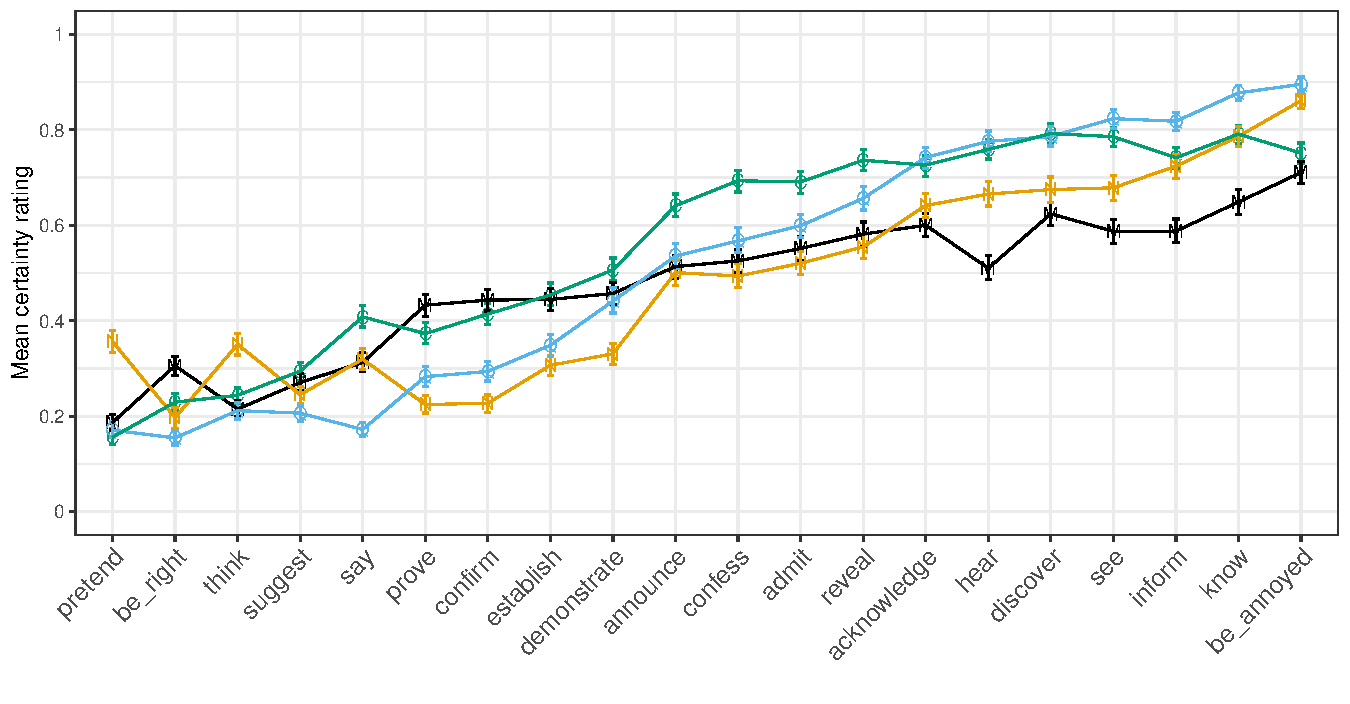
\includegraphics[width=\textwidth]{graphs/proj-by-both.pdf}}\vspace{-1.8\baselineskip}
	\caption{\small Mean certainty ratings by predicate and operator with 95\% bootstrapped confidence intervals. Embedding operator coded by letter and color:  \texttt{N} (orange): negation, \texttt{M} (black): modals, \texttt{C} (green): conditional antecedents, \texttt{Q} (blue): polar questions.}
	\label{fig:figure1}
\end{figure}

\begin{table}[h]
	\vspace{-1\baselineskip}\phantom{.}
	\centering
	% \hspace{-1.2em}
	\begin{tabular}{p{.65\linewidth} p{.3\linewidth}}
		\scalebox{.72}{
			\begin{tabular}{llrrrr}
				Model & & Estimate & Std. Error & t-value\\
				\midrule
				\#1 & Intercept: \emph{\bf be annoyed}/negation & 0.87 & 0.01  & 75.8 & *** \\
				& operator: conditional & -0.12 & 0.02  & -7.38 & *** \\
				& operator: modal & -0.16 & 0.02  & -10.04 & *** \\
				& operator: question & 0.02 & 0.01  & 1.74 & n.s. \\
				\midrule
				\#2 & Intercept: \emph{\bf know}/negation & 0.79 & 0.01 &  69.24 & *** \\
				&		operator: conditional & -0.001 & 0.02  & -0.08 & n.s. \\
				&		operator: modal  & -0.14 & 0.02  & -9.2 & *** \\
				&		operator: question & 0.08 & 0.01  & 5.72 & *** \\
				\midrule
				\#3 & Intercept: \emph{\bf discover}/negation & 0.68 & 0.01  & 59.48 & *** \\
				& operator: conditional & 0.11 & 0.02  & 7.11 & *** \\
				&		operator: modal & -0.06 & 0.02  & -3.6 & *** \\
				&		operator: question & 0.1 & 0.01  & 7.07 & *** \\

				\bottomrule
			\end{tabular}
		}
		&
		\parbox{\linewidth}{\caption{\small Relevant parts of three linear mixed effects models that predict certainty ratings from a fixed effect of operator, predicate, and their interaction, with random effects for participant and CC. Models were fit with \texttt{lme4, lmertest} in \texttt{R}.}\label{t:models}}

	\end{tabular}
\end{table}

\hspace{-2.7em}
	\begin{minipage}{\textwidth}\centering
	\begin{tabular}{p{.235\linewidth} p{.235\linewidth} p{.235\linewidth} p{.235\linewidth}}
		\parbox{\linewidth}{\centering (a) \textbf{Negation high}\\
		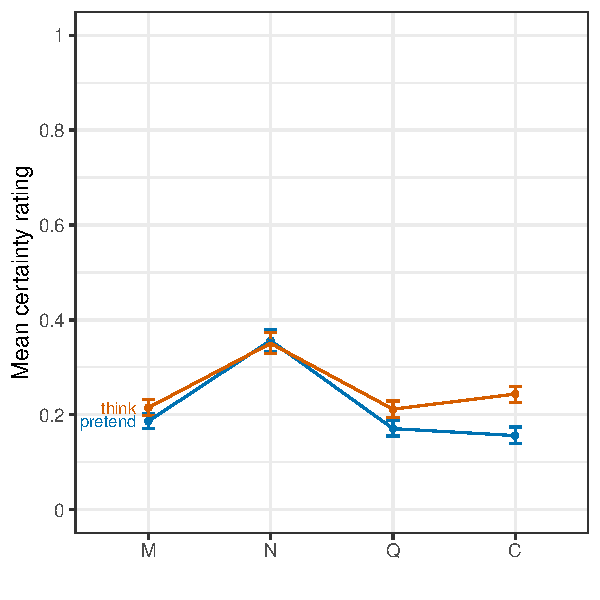
\includegraphics[width=.26\textwidth]{graphs/profile1.pdf}}
		&
		\parbox{\linewidth}{\centering (b) \textbf{Negation low}\\
		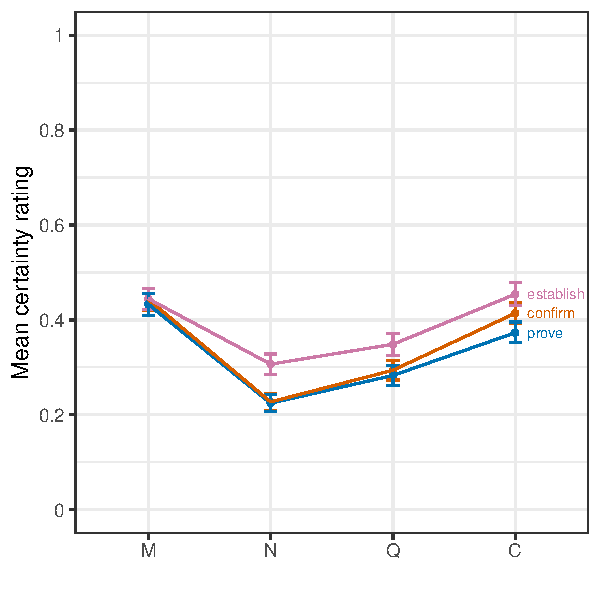
\includegraphics[width=.26\textwidth]{graphs/profile4.pdf}}
		&
		\parbox{\linewidth}{\centering (c) \textbf{Conditional high}\\
		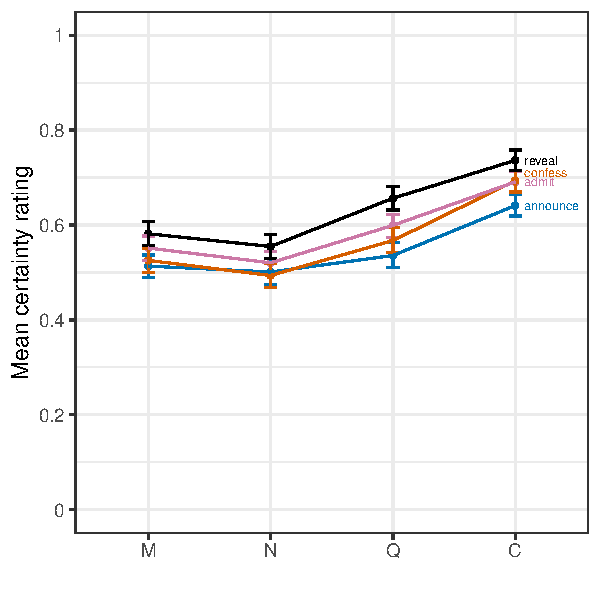
\includegraphics[width=.26\textwidth]{graphs/profile2.pdf}}
		&
		\parbox{\linewidth}{\centering (d) \textbf{Modal low}\\
		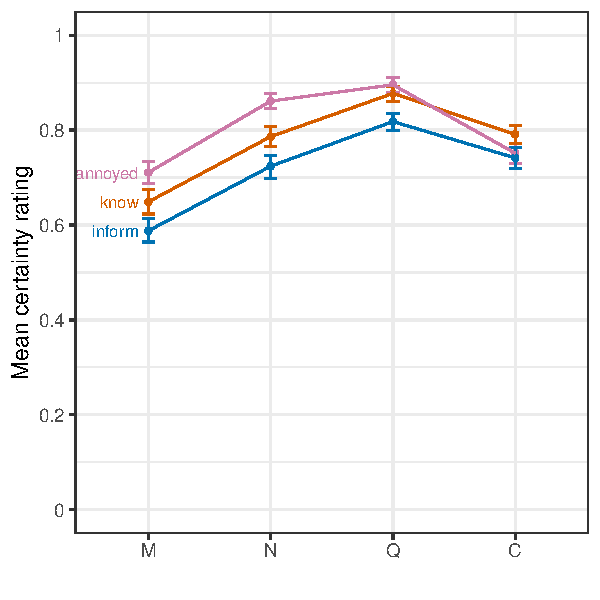
\includegraphics[width=.26\textwidth]{graphs/profile5.pdf}}
	\end{tabular}
\end{minipage}

\vspace{-.4\baselineskip}
\noindent \normalsize Figure 2: \small Mean certainty ratings by operator (\texttt{M}: Modal, \texttt{N}: Negation, \texttt{Q}: Polar Question, \texttt{C}: Conditional antecedent) with 95\% bootstrapped confidence intervals, for some groups of predicates (\lq predicate patterns\rq).

% \begin{figure}[h]
% 	\hspace{-2.5em}
	
% 	\vspace{-\baselineskip}
% 	% \caption{Mean certainty-ratings by operator for four predicate patterns in our data.}
% 	\label{fig:figure2}
% \end{figure}

\newpage

% \begin{table}[ht]
% 	\caption{Model output w \texttt{be\_annoyed/n} as baseline}
% 	\label{tab:annoyed-n}
% 	\centering

% 	\begin{tabular}{lrrrrr}
% 		\toprule
% 		  & Estimate & Std. Error & df & t value & Pr(>|t|)\\
% 		\midrule
% 		(Intercept) & 0.8669958 & 0.0114402 & 1479.204 & 75.7850523 & 0.0000000\\
% 		opc & -0.1155850 & 0.0156641 & 26227.368 & -7.3789836 & 0.0000000\\
% 		opm & -0.1564480 & 0.0155858 & 26288.139 & -10.0378702 & 0.0000000\\
% 		opq & 0.0249138 & 0.0143090 & 56826.915 & 1.7411232 & 0.0816674\\
% 		verbsuggest & -0.6162683 & 0.0134941 & 54372.895 & -45.6694112 & 0.0000000\\
% 		\addlinespace
% 		verbacknowledge & -0.2204417 & 0.0134948 & 54373.777 & -16.3352724 & 0.0000000\\
% 		verbadmit & -0.3402430 & 0.0134933 & 54371.874 & -25.2156750 & 0.0000000\\
% 		verbannounce & -0.3607504 & 0.0134931 & 54371.547 & -26.7359958 & 0.0000000\\
% 		verbbe\_right & -0.6638924 & 0.0134936 & 54372.293 & -49.2003974 & 0.0000000\\
% 		verbconfess & -0.3681695 & 0.0134949 & 54373.904 & -27.2820517 & 0.0000000\\
% 		\addlinespace
% 		verbconfirm & -0.6338363 & 0.0134931 & 54371.657 & -46.9746939 & 0.0000000\\
% 		verbdemonstrate & -0.5307026 & 0.0134935 & 54372.157 & -39.3301466 & 0.0000000\\
% 		verbdiscover & -0.1864716 & 0.0134942 & 54372.992 & -13.8186520 & 0.0000000\\
% 		verbestablish & -0.5542561 & 0.0134933 & 54371.853 & -41.0764079 & 0.0000000\\
% 		verbhear & -0.1956794 & 0.0134938 & 54372.473 & -14.5014554 & 0.0000000\\
% 		\addlinespace
% 		verbinform & -0.1374428 & 0.0134945 & 54373.345 & -10.1851106 & 0.0000000\\
% 		verbknow & -0.0748953 & 0.0134936 & 54372.288 & -5.5504197 & 0.0000000\\
% 		verbpretend & -0.5049533 & 0.0134944 & 54373.218 & -37.4195409 & 0.0000000\\
% 		verbprove & -0.6364950 & 0.0134935 & 54372.138 & -47.1704273 & 0.0000000\\
% 		verbreveal & -0.3057814 & 0.0134937 & 54372.418 & -22.6609884 & 0.0000000\\
% 		\addlinespace
% 		verbsay & -0.5419725 & 0.0134925 & 54370.770 & -40.1685159 & 0.0000000\\
% 		verbsee & -0.1827512 & 0.0134932 & 54371.791 & -13.5438968 & 0.0000000\\
% 		verbthink & -0.5101198 & 0.0134930 & 54371.491 & -37.8062103 & 0.0000000\\
% 		opc:verbsuggest & 0.1594325 & 0.0190634 & 54372.626 & 8.3632939 & 0.0000000\\
% 		opm:verbsuggest & 0.1766113 & 0.0189718 & 54372.046 & 9.3091498 & 0.0000000\\
% 		\addlinespace
% 		opq:verbsuggest & -0.0737648 & 0.0192906 & 54372.717 & -3.8238781 & 0.0001315\\
% 		opc:verbacknowledge & 0.1945569 & 0.0190630 & 54372.333 & 10.2059764 & 0.0000000\\
% 		opm:verbacknowledge & 0.1100553 & 0.0189729 & 54373.070 & 5.8006461 & 0.0000000\\
% 		opq:verbacknowledge & 0.0672935 & 0.0192909 & 54372.991 & 3.4883599 & 0.0004864\\
% 		opc:verbadmit & 0.2803349 & 0.0190626 & 54371.933 & 14.7060204 & 0.0000000\\
% 		\addlinespace
% 		opm:verbadmit & 0.1810708 & 0.0189717 & 54371.994 & 9.5442376 & 0.0000000\\
% 		opq:verbadmit & 0.0440050 & 0.0192896 & 54371.832 & 2.2812856 & 0.0225354\\
% 		opc:verbannounce & 0.2503929 & 0.0190639 & 54373.132 & 13.1343759 & 0.0000000\\
% 		opm:verbannounce & 0.1633026 & 0.0189721 & 54372.338 & 8.6075049 & 0.0000000\\
% 		opq:verbannounce & 0.0017532 & 0.0192899 & 54372.121 & 0.0908892 & 0.9275810\\
% 		\addlinespace
% 		opc:verbbe\_right & 0.1424317 & 0.0190623 & 54371.698 & 7.4718895 & 0.0000000\\
% 		opm:verbbe\_right & 0.2582399 & 0.0189717 & 54371.967 & 13.6118412 & 0.0000000\\
% 		opq:verbbe\_right & -0.0776846 & 0.0192897 & 54371.974 & -4.0272512 & 0.0000565\\
% 		opc:verbconfess & 0.3111230 & 0.0190643 & 54373.455 & 16.3196605 & 0.0000000\\
% 		opm:verbconfess & 0.1837114 & 0.0189741 & 54374.125 & 9.6821973 & 0.0000000\\
% 		\addlinespace
% 		opq:verbconfess & 0.0393640 & 0.0192890 & 54371.320 & 2.0407459 & 0.0412809\\
% 		opc:verbconfirm & 0.2963833 & 0.0190629 & 54372.237 & 15.5476205 & 0.0000000\\
% 		opm:verbconfirm & 0.3663333 & 0.0189721 & 54372.324 & 19.3090505 & 0.0000000\\
% 		opq:verbconfirm & 0.0312870 & 0.0192902 & 54372.377 & 1.6219108 & 0.1048282\\
% 		opc:verbdemonstrate & 0.2854366 & 0.0190647 & 54373.829 & 14.9719656 & 0.0000000\\
% 		\addlinespace
% 		opm:verbdemonstrate & 0.2783816 & 0.0189716 & 54371.830 & 14.6736292 & 0.0000000\\
% 		opq:verbdemonstrate & 0.0753554 & 0.0192892 & 54371.520 & 3.9066023 & 0.0000937\\
% 		opc:verbdiscover & 0.2270099 & 0.0190632 & 54372.450 & 11.9082962 & 0.0000000\\
% 		opm:verbdiscover & 0.1002424 & 0.0189726 & 54372.795 & 5.2835252 & 0.0000001\\
% 		opq:verbdiscover & 0.0762282 & 0.0192898 & 54372.014 & 3.9517423 & 0.0000777\\
% 		\addlinespace
% 		opc:verbestablish & 0.2570817 & 0.0190633 & 54372.539 & 13.4857080 & 0.0000000\\
% 		opm:verbestablish & 0.2879581 & 0.0189714 & 54371.677 & 15.1785426 & 0.0000000\\
% 		opq:verbestablish & 0.0061604 & 0.0192893 & 54371.583 & 0.3193687 & 0.7494481\\
% 		opc:verbhear & 0.2016309 & 0.0190630 & 54372.273 & 10.5770983 & 0.0000000\\
% 		opm:verbhear & -0.0046313 & 0.0189714 & 54371.681 & -0.2441216 & 0.8071376\\
% 		\addlinespace
% 		opq:verbhear & 0.0756021 & 0.0192902 & 54372.373 & 3.9192008 & 0.0000890\\
% 		opc:verbinform & 0.1278740 & 0.0190645 & 54373.631 & 6.7074362 & 0.0000000\\
% 		opm:verbinform & 0.0141486 & 0.0189741 & 54374.122 & 0.7456761 & 0.4558664\\
% 		opq:verbinform & 0.0587564 & 0.0192913 & 54373.322 & 3.0457537 & 0.0023221\\
% 		opc:verbknow & 0.1142699 & 0.0190629 & 54372.206 & 5.9943629 & 0.0000000\\
% 		\addlinespace
% 		opm:verbknow & 0.0130032 & 0.0189709 & 54371.181 & 0.6854301 & 0.4930755\\
% 		opq:verbknow & 0.0569598 & 0.0192897 & 54371.975 & 2.9528579 & 0.0031498\\
% 		opc:verbpretend & -0.0902047 & 0.0190640 & 54373.155 & -4.7316842 & 0.0000022\\
% 		opm:verbpretend & -0.0194245 & 0.0189738 & 54373.822 & -1.0237558 & 0.3059552\\
% 		opq:verbpretend & -0.2196823 & 0.0192900 & 54372.250 & -11.3883795 & 0.0000000\\
% 		\addlinespace
% 		opc:verbprove & 0.2579585 & 0.0190627 & 54372.031 & 13.5320999 & 0.0000000\\
% 		opm:verbprove & 0.3580525 & 0.0189720 & 54372.223 & 18.8726898 & 0.0000000\\
% 		opq:verbprove & 0.0230805 & 0.0192908 & 54372.899 & 1.1964509 & 0.2315259\\
% 		opc:verbreveal & 0.2902650 & 0.0190644 & 54373.511 & 15.2255216 & 0.0000000\\
% 		opm:verbreveal & 0.1767476 & 0.0189723 & 54372.513 & 9.3160804 & 0.0000000\\
% 		\addlinespace
% 		opq:verbreveal & 0.0665887 & 0.0192906 & 54372.717 & 3.4518763 & 0.0005571\\
% 		opc:verbsay & 0.1985351 & 0.0190618 & 54371.193 & 10.4153412 & 0.0000000\\
% 		opm:verbsay & 0.1451974 & 0.0189723 & 54372.495 & 7.6531273 & 0.0000000\\
% 		opq:verbsay & -0.1815738 & 0.0192889 & 54371.195 & -9.4133926 & 0.0000000\\
% 		opc:verbsee & 0.2175191 & 0.0190629 & 54372.234 & 11.4105822 & 0.0000000\\
% 		\addlinespace
% 		opm:verbsee & 0.0594092 & 0.0189723 & 54372.499 & 3.1313655 & 0.0017409\\
% 		opq:verbsee & 0.1108274 & 0.0192896 & 54371.840 & 5.7454526 & 0.0000000\\
% 		opc:verbthink & 0.0023197 & 0.0190619 & 54371.272 & 0.1216913 & 0.9031440\\
% 		opm:verbthink & 0.0145577 & 0.0189717 & 54371.965 & 0.7673367 & 0.4428847\\
% 		opq:verbthink & -0.1738342 & 0.0192903 & 54372.438 & -9.0115053 & 0.0000000\\
% 		\bottomrule
% 	\end{tabular}
% \end{table}

% \newpage

% \begin{table}[ht]
% 	\caption{Model output w \texttt{discover/n} as baseline}
% 	\label{tab:discover-n}
% 	\centering

% 	\begin{tabular}{lrrrrr}
% 		\toprule
% 		  & Estimate & Std. Error & df & t value & Pr(>|t|)\\
% 		\midrule
% 		(Intercept) & 0.6805242 & 0.0114403 & 1479.217 & 59.4849565 & 0.0000000\\
% 		opc & 0.1114249 & 0.0156639 & 26226.686 & 7.1134644 & 0.0000000\\
% 		opm & -0.0562056 & 0.0155855 & 26286.826 & -3.6062779 & 0.0003112\\
% 		opq & 0.1011420 & 0.0143103 & 56828.295 & 7.0677830 & 0.0000000\\
% 		verbbe\_annoyed & 0.1864716 & 0.0134942 & 54372.998 & 13.8186521 & 0.0000000\\
% 		\addlinespace
% 		verbsuggest & -0.4297967 & 0.0134937 & 54372.361 & -31.8516905 & 0.0000000\\
% 		verbacknowledge & -0.0339702 & 0.0134936 & 54372.308 & -2.5174950 & 0.0118221\\
% 		verbadmit & -0.1537714 & 0.0134942 & 54372.985 & -11.3953857 & 0.0000000\\
% 		verbannounce & -0.1742788 & 0.0134947 & 54373.649 & -12.9145926 & 0.0000000\\
% 		verbbe\_right & -0.4774208 & 0.0134935 & 54372.079 & -35.3816304 & 0.0000000\\
% 		\addlinespace
% 		verbconfess & -0.1816980 & 0.0134936 & 54372.192 & -13.4655376 & 0.0000000\\
% 		verbconfirm & -0.4473648 & 0.0134944 & 54373.311 & -33.1517710 & 0.0000000\\
% 		verbdemonstrate & -0.3442310 & 0.0134928 & 54371.247 & -25.5121517 & 0.0000000\\
% 		verbestablish & -0.3677846 & 0.0134928 & 54371.167 & -27.2579106 & 0.0000000\\
% 		verbhear & -0.0092079 & 0.0134940 & 54372.798 & -0.6823676 & 0.4950095\\
% 		\addlinespace
% 		verbinform & 0.0490288 & 0.0134942 & 54373.066 & 3.6333114 & 0.0002801\\
% 		verbknow & 0.1115762 & 0.0134931 & 54371.668 & 8.2691029 & 0.0000000\\
% 		verbpretend & -0.3184818 & 0.0134943 & 54373.176 & -23.6011440 & 0.0000000\\
% 		verbprove & -0.4500234 & 0.0134934 & 54372.042 & -33.3512833 & 0.0000000\\
% 		verbreveal & -0.1193099 & 0.0134941 & 54372.880 & -8.8416323 & 0.0000000\\
% 		\addlinespace
% 		verbsay & -0.3555009 & 0.0134943 & 54373.168 & -26.3444678 & 0.0000000\\
% 		verbsee & 0.0037204 & 0.0134930 & 54371.450 & 0.2757288 & 0.7827574\\
% 		verbthink & -0.3236483 & 0.0134936 & 54372.197 & -23.9853913 & 0.0000000\\
% 		opc:verbbe\_annoyed & -0.2270099 & 0.0190632 & 54372.453 & -11.9082963 & 0.0000000\\
% 		opm:verbbe\_annoyed & -0.1002424 & 0.0189726 & 54372.798 & -5.2835253 & 0.0000001\\
% 		\addlinespace
% 		opq:verbbe\_annoyed & -0.0762282 & 0.0192898 & 54372.017 & -3.9517423 & 0.0000777\\
% 		opc:verbsuggest & -0.0675773 & 0.0190625 & 54371.851 & -3.5450396 & 0.0003929\\
% 		opm:verbsuggest & 0.0763690 & 0.0189709 & 54371.211 & 4.0255864 & 0.0000569\\
% 		opq:verbsuggest & -0.1499930 & 0.0192910 & 54373.069 & -7.7752981 & 0.0000000\\
% 		opc:verbacknowledge & -0.0324529 & 0.0190617 & 54371.116 & -1.7025196 & 0.0886637\\
% 		\addlinespace
% 		opm:verbacknowledge & 0.0098129 & 0.0189711 & 54371.417 & 0.5172570 & 0.6049789\\
% 		opq:verbacknowledge & -0.0089347 & 0.0192902 & 54372.396 & -0.4631724 & 0.6432426\\
% 		opc:verbadmit & 0.0533251 & 0.0190632 & 54372.508 & 2.7972739 & 0.0051554\\
% 		opm:verbadmit & 0.0808284 & 0.0189728 & 54372.916 & 4.2602367 & 0.0000205\\
% 		opq:verbadmit & -0.0322232 & 0.0192908 & 54372.883 & -1.6703960 & 0.0948468\\
% 		\addlinespace
% 		opc:verbannounce & 0.0233831 & 0.0190642 & 54373.367 & 1.2265427 & 0.2199998\\
% 		opm:verbannounce & 0.0630602 & 0.0189726 & 54372.754 & 3.3237576 & 0.0008887\\
% 		opq:verbannounce & -0.0744750 & 0.0192926 & 54374.465 & -3.8602856 & 0.0001134\\
% 		opc:verbbe\_right & -0.0845782 & 0.0190620 & 54371.360 & -4.4370099 & 0.0000091\\
% 		opm:verbbe\_right & 0.1579976 & 0.0189719 & 54372.163 & 8.3279685 & 0.0000000\\
% 		\addlinespace
% 		opq:verbbe\_right & -0.1539128 & 0.0192901 & 54372.283 & -7.9788617 & 0.0000000\\
% 		opc:verbconfess & 0.0841131 & 0.0190632 & 54372.437 & 4.4123417 & 0.0000102\\
% 		opm:verbconfess & 0.0834691 & 0.0189719 & 54372.142 & 4.3996174 & 0.0000109\\
% 		opq:verbconfess & -0.0368642 & 0.0192905 & 54372.632 & -1.9110088 & 0.0560087\\
% 		opc:verbconfirm & 0.0693734 & 0.0190644 & 54373.529 & 3.6388992 & 0.0002741\\
% 		\addlinespace
% 		opm:verbconfirm & 0.2660910 & 0.0189728 & 54372.917 & 14.0248948 & 0.0000000\\
% 		opq:verbconfirm & -0.0449413 & 0.0192914 & 54373.472 & -2.3295974 & 0.0198311\\
% 		opc:verbdemonstrate & 0.0584268 & 0.0190633 & 54372.586 & 3.0648793 & 0.0021786\\
% 		opm:verbdemonstrate & 0.1781393 & 0.0189714 & 54371.707 & 9.3898743 & 0.0000000\\
% 		opq:verbdemonstrate & -0.0008729 & 0.0192906 & 54372.707 & -0.0452486 & 0.9639093\\
% 		\addlinespace
% 		opc:verbestablish & 0.0300718 & 0.0190618 & 54371.161 & 1.5775980 & 0.1146638\\
% 		opm:verbestablish & 0.1877158 & 0.0189720 & 54372.212 & 9.8943713 & 0.0000000\\
% 		opq:verbestablish & -0.0700678 & 0.0192899 & 54372.103 & -3.6323635 & 0.0002811\\
% 		opc:verbhear & -0.0253789 & 0.0190637 & 54372.970 & -1.3312665 & 0.1831069\\
% 		opm:verbhear & -0.1048737 & 0.0189721 & 54372.368 & -5.5277707 & 0.0000000\\
% 		\addlinespace
% 		opq:verbhear & -0.0006261 & 0.0192909 & 54372.991 & -0.0324581 & 0.9741069\\
% 		opc:verbinform & -0.0991359 & 0.0190633 & 54372.605 & -5.2003420 & 0.0000002\\
% 		opm:verbinform & -0.0860938 & 0.0189733 & 54373.368 & -4.5376355 & 0.0000057\\
% 		opq:verbinform & -0.0174718 & 0.0192931 & 54374.843 & -0.9055994 & 0.3651520\\
% 		opc:verbknow & -0.1127399 & 0.0190628 & 54372.127 & -5.9141311 & 0.0000000\\
% 		\addlinespace
% 		opm:verbknow & -0.0872392 & 0.0189719 & 54372.149 & -4.5983336 & 0.0000043\\
% 		opq:verbknow & -0.0192684 & 0.0192895 & 54371.814 & -0.9989027 & 0.3178463\\
% 		opc:verbpretend & -0.3172145 & 0.0190639 & 54373.134 & -16.6395086 & 0.0000000\\
% 		opm:verbpretend & -0.1196669 & 0.0189725 & 54372.658 & -6.3073967 & 0.0000000\\
% 		opq:verbpretend & -0.2959105 & 0.0192916 & 54373.627 & -15.3388172 & 0.0000000\\
% 		\addlinespace
% 		opc:verbprove & 0.0309486 & 0.0190626 & 54371.908 & 1.6235265 & 0.1044827\\
% 		opm:verbprove & 0.2578102 & 0.0189728 & 54372.987 & 13.5883819 & 0.0000000\\
% 		opq:verbprove & -0.0531478 & 0.0192907 & 54372.839 & -2.7550974 & 0.0058694\\
% 		opc:verbreveal & 0.0632551 & 0.0190641 & 54373.234 & 3.3180321 & 0.0009071\\
% 		opm:verbreveal & 0.0765052 & 0.0189711 & 54371.383 & 4.0327309 & 0.0000552\\
% 		\addlinespace
% 		opq:verbreveal & -0.0096396 & 0.0192917 & 54373.669 & -0.4996755 & 0.6173056\\
% 		opc:verbsay & -0.0284748 & 0.0190633 & 54372.590 & -1.4936938 & 0.1352615\\
% 		opm:verbsay & 0.0449550 & 0.0189713 & 54371.586 & 2.3696339 & 0.0178092\\
% 		opq:verbsay & -0.2578020 & 0.0192911 & 54373.227 & -13.3637456 & 0.0000000\\
% 		opc:verbsee & -0.0094907 & 0.0190633 & 54372.613 & -0.4978528 & 0.6185898\\
% 		\addlinespace
% 		opm:verbsee & -0.0408332 & 0.0189714 & 54371.728 & -2.1523480 & 0.0313743\\
% 		opq:verbsee & 0.0345992 & 0.0192916 & 54373.623 & 1.7934827 & 0.0729013\\
% 		opc:verbthink & -0.2246902 & 0.0190628 & 54372.159 & -11.7868151 & 0.0000000\\
% 		opm:verbthink & -0.0856847 & 0.0189719 & 54372.175 & -4.5163904 & 0.0000063\\
% 		opq:verbthink & -0.2500624 & 0.0192911 & 54373.178 & -12.9625865 & 0.0000000\\
% 		\bottomrule
% 	\end{tabular}
% \end{table}

% \newpage

% \begin{table}[ht]
% 	\caption{Model output w \texttt{know/n} as baseline}
% 	\label{tab:discover-n}
% 	\centering

% 	\begin{tabular}{lrrrrr}
% 		\toprule
% 		  & Estimate & Std. Error & df & t value & Pr(>|t|)\\
% 		\midrule
% 		(Intercept) & 0.7921005 & 0.0114401 & 1479.182 & 69.2391632 & 0.0000000\\
% 		opc & -0.0013151 & 0.0156638 & 26226.099 & -0.0839558 & 0.9330922\\
% 		opm & -0.1434448 & 0.0155855 & 26286.727 & -9.2037503 & 0.0000000\\
% 		opq & 0.0818736 & 0.0143093 & 56827.205 & 5.7217106 & 0.0000000\\
% 		verbdiscover & -0.1115762 & 0.0134931 & 54371.661 & -8.2691029 & 0.0000000\\
% 		\addlinespace
% 		verbbe\_annoyed & 0.0748953 & 0.0134936 & 54372.286 & 5.5504198 & 0.0000000\\
% 		verbsuggest & -0.5413729 & 0.0134928 & 54371.215 & -40.1230775 & 0.0000000\\
% 		verbacknowledge & -0.1455464 & 0.0134940 & 54372.778 & -10.7859911 & 0.0000000\\
% 		verbadmit & -0.2653476 & 0.0134936 & 54372.243 & -19.6647018 & 0.0000000\\
% 		verbannounce & -0.2858550 & 0.0134935 & 54372.051 & -21.1847253 & 0.0000000\\
% 		\addlinespace
% 		verbbe\_right & -0.5889971 & 0.0134936 & 54372.234 & -43.6501264 & 0.0000000\\
% 		verbconfess & -0.2932742 & 0.0134933 & 54371.896 & -21.7347532 & 0.0000000\\
% 		verbconfirm & -0.5589410 & 0.0134943 & 54373.134 & -41.4204989 & 0.0000000\\
% 		verbdemonstrate & -0.4558072 & 0.0134931 & 54371.605 & -33.7807521 & 0.0000000\\
% 		verbestablish & -0.4793608 & 0.0134938 & 54372.501 & -35.5245129 & 0.0000000\\
% 		\addlinespace
% 		verbhear & -0.1207841 & 0.0134931 & 54371.608 & -8.9515418 & 0.0000000\\
% 		verbinform & -0.0625474 & 0.0134940 & 54372.811 & -4.6351853 & 0.0000036\\
% 		verbpretend & -0.4300580 & 0.0134939 & 54372.685 & -31.8704317 & 0.0000000\\
% 		verbprove & -0.5615997 & 0.0134934 & 54372.014 & -41.6202578 & 0.0000000\\
% 		verbreveal & -0.2308861 & 0.0134943 & 54373.179 & -17.1098402 & 0.0000000\\
% 		\addlinespace
% 		verbsay & -0.4670771 & 0.0134939 & 54372.578 & -34.6140392 & 0.0000000\\
% 		verbsee & -0.1078558 & 0.0134932 & 54371.715 & -7.9933523 & 0.0000000\\
% 		verbthink & -0.4352245 & 0.0134933 & 54371.896 & -32.2547883 & 0.0000000\\
% 		opc:verbdiscover & 0.1127399 & 0.0190628 & 54372.122 & 5.9141311 & 0.0000000\\
% 		opm:verbdiscover & 0.0872392 & 0.0189719 & 54372.145 & 4.5983336 & 0.0000043\\
% 		\addlinespace
% 		opq:verbdiscover & 0.0192684 & 0.0192895 & 54371.810 & 0.9989027 & 0.3178463\\
% 		opc:verbbe\_annoyed & -0.1142699 & 0.0190629 & 54372.206 & -5.9943630 & 0.0000000\\
% 		opm:verbbe\_annoyed & -0.0130032 & 0.0189709 & 54371.180 & -0.6854301 & 0.4930755\\
% 		opq:verbbe\_annoyed & -0.0569598 & 0.0192897 & 54371.974 & -2.9528580 & 0.0031498\\
% 		opc:verbsuggest & 0.0451626 & 0.0190614 & 54370.865 & 2.3693169 & 0.0178244\\
% 		\addlinespace
% 		opm:verbsuggest & 0.1636081 & 0.0189713 & 54371.561 & 8.6239932 & 0.0000000\\
% 		opq:verbsuggest & -0.1307246 & 0.0192896 & 54371.847 & -6.7769511 & 0.0000000\\
% 		opc:verbacknowledge & 0.0802870 & 0.0190639 & 54373.059 & 4.2114778 & 0.0000254\\
% 		opm:verbacknowledge & 0.0970521 & 0.0189731 & 54373.215 & 5.1152465 & 0.0000003\\
% 		opq:verbacknowledge & 0.0103337 & 0.0192900 & 54372.183 & 0.5357031 & 0.5921659\\
% 		\addlinespace
% 		opc:verbadmit & 0.1660650 & 0.0190633 & 54372.568 & 8.7112405 & 0.0000000\\
% 		opm:verbadmit & 0.1680676 & 0.0189725 & 54372.674 & 8.8584875 & 0.0000000\\
% 		opq:verbadmit & -0.0129548 & 0.0192897 & 54371.901 & -0.6715939 & 0.5018451\\
% 		opc:verbannounce & 0.1361230 & 0.0190629 & 54372.249 & 7.1407107 & 0.0000000\\
% 		opm:verbannounce & 0.1502994 & 0.0189716 & 54371.859 & 7.9223393 & 0.0000000\\
% 		\addlinespace
% 		opq:verbannounce & -0.0552066 & 0.0192897 & 54371.911 & -2.8619784 & 0.0042117\\
% 		opc:verbbe\_right & 0.0281618 & 0.0190625 & 54371.883 & 1.4773357 & 0.1395915\\
% 		opm:verbbe\_right & 0.2452367 & 0.0189720 & 54372.236 & 12.9262410 & 0.0000000\\
% 		opq:verbbe\_right & -0.1346444 & 0.0192901 & 54372.308 & -6.9799743 & 0.0000000\\
% 		opc:verbconfess & 0.1968531 & 0.0190627 & 54372.016 & 10.3266157 & 0.0000000\\
% 		\addlinespace
% 		opm:verbconfess & 0.1707082 & 0.0189737 & 54373.731 & 8.9971020 & 0.0000000\\
% 		opq:verbconfess & -0.0175959 & 0.0192891 & 54371.441 & -0.9122160 & 0.3616590\\
% 		opc:verbconfirm & 0.1821133 & 0.0190626 & 54371.955 & 9.5534239 & 0.0000000\\
% 		opm:verbconfirm & 0.3533301 & 0.0189718 & 54372.046 & 18.6239655 & 0.0000000\\
% 		opq:verbconfirm & -0.0256729 & 0.0192917 & 54373.707 & -1.3307729 & 0.1832693\\
% 		\addlinespace
% 		opc:verbdemonstrate & 0.1711667 & 0.0190647 & 54373.791 & 8.9782020 & 0.0000000\\
% 		opm:verbdemonstrate & 0.2653784 & 0.0189716 & 54371.911 & 13.9881581 & 0.0000000\\
% 		opq:verbdemonstrate & 0.0183955 & 0.0192903 & 54372.499 & 0.9536136 & 0.3402835\\
% 		opc:verbestablish & 0.1428117 & 0.0190634 & 54372.667 & 7.4914038 & 0.0000000\\
% 		opm:verbestablish & 0.2749549 & 0.0189719 & 54372.156 & 14.4927310 & 0.0000000\\
% 		\addlinespace
% 		opq:verbestablish & -0.0507994 & 0.0192892 & 54371.529 & -2.6335636 & 0.0084518\\
% 		opc:verbhear & 0.0873610 & 0.0190622 & 54371.557 & 4.5829467 & 0.0000046\\
% 		opm:verbhear & -0.0176345 & 0.0189709 & 54371.193 & -0.9295579 & 0.3526042\\
% 		opq:verbhear & 0.0186422 & 0.0192902 & 54372.432 & 0.9664076 & 0.3338446\\
% 		opc:verbinform & 0.0136041 & 0.0190628 & 54372.117 & 0.7136441 & 0.4754504\\
% 		\addlinespace
% 		opm:verbinform & 0.0011454 & 0.0189738 & 54373.859 & 0.0603655 & 0.9518647\\
% 		opq:verbinform & 0.0017966 & 0.0192921 & 54374.044 & 0.0931259 & 0.9258039\\
% 		opc:verbpretend & -0.2044746 & 0.0190640 & 54373.227 & -10.7256652 & 0.0000000\\
% 		opm:verbpretend & -0.0324277 & 0.0189726 & 54372.773 & -1.7091875 & 0.0874219\\
% 		opq:verbpretend & -0.2766421 & 0.0192909 & 54373.044 & -14.3405213 & 0.0000000\\
% 		\addlinespace
% 		opc:verbprove & 0.1436885 & 0.0190622 & 54371.604 & 7.5378609 & 0.0000000\\
% 		opm:verbprove & 0.3450493 & 0.0189712 & 54371.500 & 18.1880552 & 0.0000000\\
% 		opq:verbprove & -0.0338794 & 0.0192909 & 54373.040 & -1.7562330 & 0.0790543\\
% 		opc:verbreveal & 0.1759951 & 0.0190637 & 54372.960 & 9.2319255 & 0.0000000\\
% 		opm:verbreveal & 0.1637444 & 0.0189722 & 54372.374 & 8.6307727 & 0.0000000\\
% 		\addlinespace
% 		opq:verbreveal & 0.0096288 & 0.0192902 & 54372.406 & 0.4991553 & 0.6176720\\
% 		opc:verbsay & 0.0842652 & 0.0190632 & 54372.497 & 4.4203002 & 0.0000099\\
% 		opm:verbsay & 0.1321942 & 0.0189719 & 54372.094 & 6.9679113 & 0.0000000\\
% 		opq:verbsay & -0.2385336 & 0.0192898 & 54371.999 & -12.3658155 & 0.0000000\\
% 		opc:verbsee & 0.1032492 & 0.0190630 & 54372.324 & 5.4162003 & 0.0000001\\
% 		\addlinespace
% 		opm:verbsee & 0.0464060 & 0.0189718 & 54372.089 & 2.4460454 & 0.0144464\\
% 		opq:verbsee & 0.0538675 & 0.0192901 & 54372.298 & 2.7924979 & 0.0052321\\
% 		opc:verbthink & -0.1119503 & 0.0190627 & 54372.030 & -5.8727378 & 0.0000000\\
% 		opm:verbthink & 0.0015545 & 0.0189713 & 54371.557 & 0.0819391 & 0.9346955\\
% 		opq:verbthink & -0.2307940 & 0.0192903 & 54372.447 & -11.9642778 & 0.0000000\\
% 		\bottomrule
% 	\end{tabular}
% \end{table}

% \bibliography{../bibliography.bib}
\bibliography{../projective-content.bib}

\end{document}